
%(BEGIN_QUESTION)
% Copyright 2012, Tony R. Kuphaldt, released under the Creative Commons Attribution License (v 1.0)
% This means you may do almost anything with this work of mine, so long as you give me proper credit

Skygg området i dette diagrammet som representerer følgende integraler (forutsatt at hver horisontale og vertikale inndeling i diagrammet har trinnverdi 1):

$$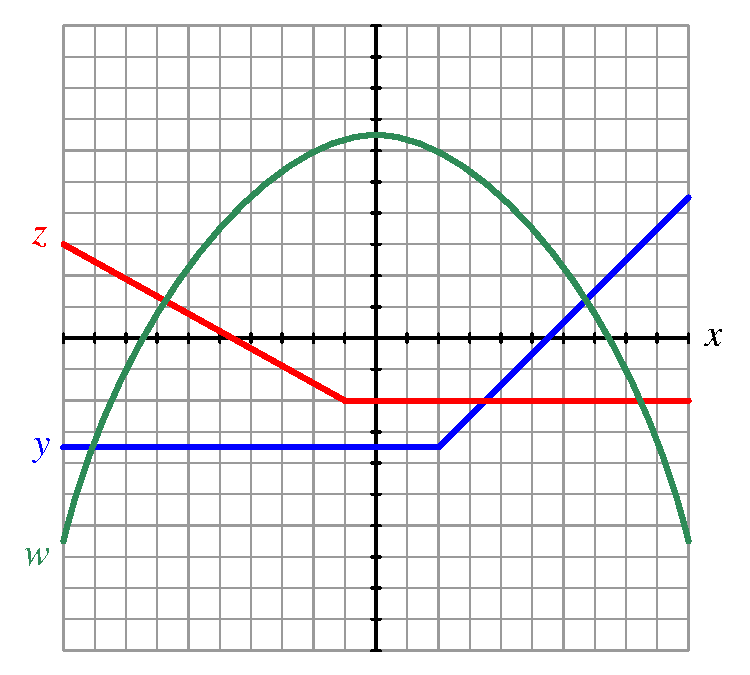
\includegraphics[width=15.5cm]{i01345x01.eps}$$

$$\int_{0}^{5} y \> dx$$

$$\int_{-1}^{-6} w \> dx$$

Avgjør også om den numeriske verdien av hvert integral er {\it positiv} eller {\it negativ}.

\underbar{file i01345}
%(END_QUESTION)





%(BEGIN_ANSWER)

Begge integralene har {\it negative} verdier:

$$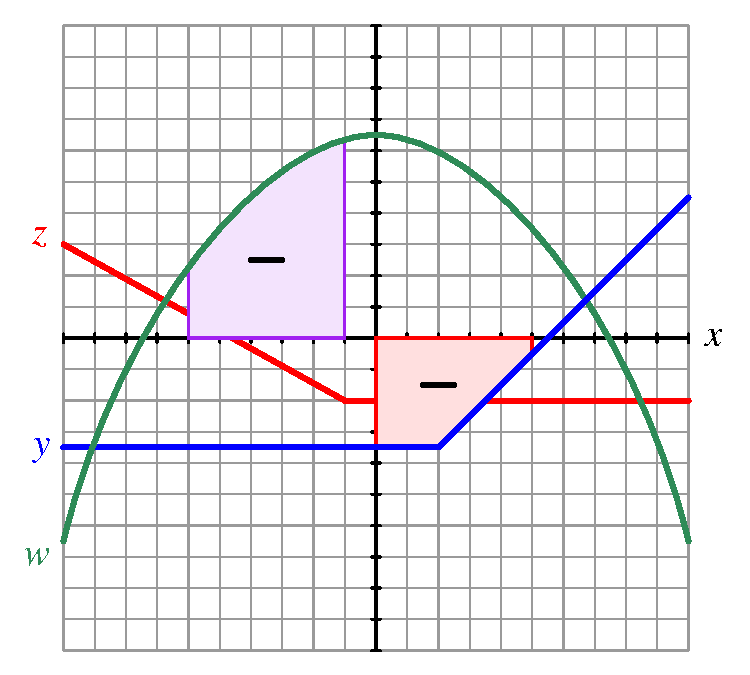
\includegraphics[width=15.5cm]{i01345x02.eps}$$

Det første integralet (skyggelagt i {\it rødt}) har positive $dx$-økninger, men negative $y$-verdier. Det andre integralet (skyggelagt i {\it fiolett}) har negative $dx$-økninger og positive $w$-verdier.

%(END_ANSWER)





%(BEGIN_NOTES)


%INDEX% Mathematics, calculus: integral (defined in a graphical sense)

%(END_NOTES)

